\documentclass{intech}
\usepackage{float}
%\usepackage{your_package}	%if you need custom package
%\usepackage[notquote]{hanging}


% * CHAPTER NUMBER * BOOK NAME * AUTHOR(S) NAME *****************************
\setcounter{chapter}{0} % It will be set by technical editor.

\booktitle{Will-be-set-by-IN-TECH}%

\chaptertitle{Search via quantum walk} % You know your chapter title?

\authors{Jiangfeng Du, Chao Lei, Gan Qin, Dawei Lu and Xinhua Peng}
\affiliation{University of Science and Technology of China}
\country{China}

% uncomment the next three or six lines, when authors are from diferent university, company or country

%\secondauthors{Author(s) with another affiliation}
%\secondaffiliation{Name of the 2nd University (Company)}
%\secondcountry{2nd country}

%\thirdauthors{}
%\thirdaffiliation{}
%\thirdcountry{}

% END * CHAPTER NUMBER * BOOK NAME * AUTHOR(S) NAME *************************


\begin{document}

\maketitle

\section{Introduction }
For an unsorted database, it takes long time to find a special element, if the number of elements in the database increase, we would take times increasing proportional to the size of the database N. So far, we have not find an efficient search algorithm for this problem. The conceive of quantum computer may bring us the hope of solving many intractable problems such as factoring large numbers, discrete logarithm and the searching problems. The first quantum algorithm for searching an unsorted database is discovered by Grover, which is named as Grover algorithm (\cite{Grover97}). The Grover algorithm can search the unsorted database with a quadratic speed up, soon after that it is proved to be the fast speed up with the quantum computer. Although unlike other quantum algorithms that make exponentially speed up upon the corresponding classical algorithms, it can not prevent us to treat Grover algorithm as a elegant harvest of the quantum computer since for very large unsorted database the quadratic speed up is not a trivial achievement.Suppose a classical search needs $10^6$ steps, and 1 step costs 8.64 seconds, then the total calculation spends 100days. While the corresponding quantum search needs $10^3$ steps, and thus the total calculation spends only 0.1 day!

Besides the Grover algorithm, there is another algorithms to solve the search problem. Quantum walk is the other approach to achieve the goal, which can also achieve quadratic speed up. Furthermore, quantum walk is soon generalized to other searching problems such as element distinctness, substructure finding etc. These problems can not be solved by Grover algorithm efficiently. This is far from ending, if we know that quantum computer is still a beautiful dream, for this reason many people doubled the effort to find the search algorithm based on conventional quantum computer or quantum walk. We know that the decoherence can shatter our dream to build a quantum computer. But if we know that quantum walk may play an important role in nature, maybe some pessimism would be taken away. There are many inspiring evidences to prove the role of quantum coherence played in nature such as photosynthesis, this may strengthen our conviction to build a quantum computer, in virtue of which we can realize our search algorithms based on quantum computer or quantum walk.

In this chapter we will focus on the search algorithm based on quantum walk. The structure of this chapter is as follows, section 2 is the introduction of the quantum walk, including the coined and continues quantum walk; section 3 is the search algorithm via quantum walk, for the general searching and the special searching problems; section 4 is focused on the physical implementation of quantum walk based search algorithm using the NMR quantum computer; in section 5 we will introduce the role may be played by quantum walk in nature such as photosynthesis, in which the high efficiency of the energy transfer is still an enigma. In the section 6 the conclusion and some future direction will be showed.

\section{Quantum walk}
Random walk is know as the Markovian chain which has been applied on the algorithms generally, it was quantized after the concept of quantum computer is formed. In this section we would introduce the concept of quantum walk from the classical random walk and then the two forms of quantum walk - coined and continues quantum walk.
\subsection{Classical random walk}
In principle, the random walk can be defined on arbitrary graph. Without loss of generality, we could focus on the random walk on one dimensional lattice. Suppose there are N lattice point arrayed on a line, each labeled by a number, negative or positive, such as in Fig. \ref{myfigure1}, the lattices are labeled form -9 to 9 . At any time we can be at only one lattice point. Then we start at lattice 0 for example, we flip a coin to decide if we go to the left lattice or the right lattice, if the coin is up, we go to left, otherwise if the coin is down, we go to right, after we go to the left or the right, then we flip the coin again to decide again if we go to the left or right. So at each step we flip a coin to decide which direction to go. After \emph{T} step, we can calculate the possibility on each lattice, for an example we can see the Fig. \ref{myfigure2}. For this case we set the probability to go to each direction to 0.5, since there are only two directions. We can also set the probability different if necessary.
\begin{figure}[htb]	% h-here, t-top, b-bottom
\centering
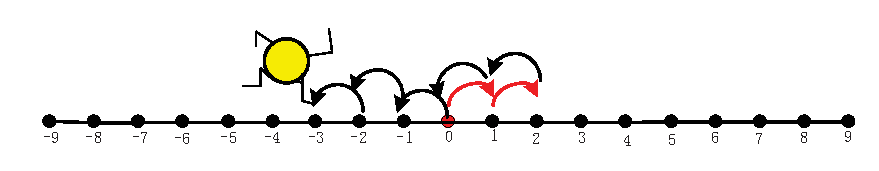
\includegraphics[width=8cm]{Fig_1} %	** if .eps don't need extension
\caption{In the case of the one dimensional lattice, a walker just has two direction to choose, in classical random walk, to decide go to left or right may be decided by a coin with two sides. This picture is from (\cite{Kendon07})}\label{myfigure1}
\end{figure}

\begin{figure}[htb]	% h-here, t-top, b-bottom
\centering
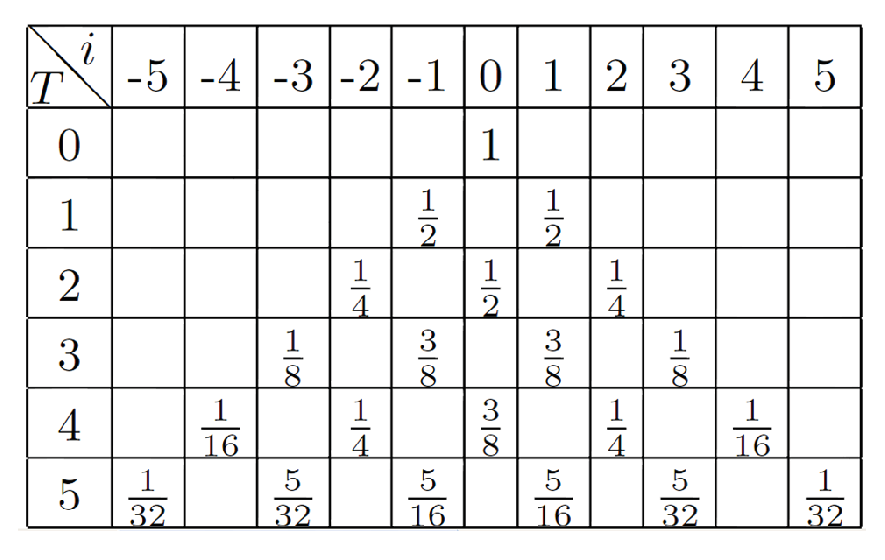
\includegraphics[width=8cm]{Fig_2} %	** if .eps don't need extension
\caption{In this picture \emph{T }is the number of step of the classical random in one dimensional lattice, $\mathrm{i}$ is the number that labels the position of the lattice, from this table we can know that after \emph{T} step of walk, the walker will be at the center (or the start place) with the max possible (\cite{Kempe03}).}\label{myfigure2}
\end{figure}

From a formal derivation we can get the probability distribution of the walker on each lattice. For a detail we can consult the book of 'A modern Course in Statistical Physics' (\cite{Reichl98}).

If we are familiar with the probability theory, when \emph{T} is large enough, it is easy to derive the probability distribution of the walker on the position is:
\begin{equation}\label{myequation1}
\rho (x,T) = \frac{1}{{\sqrt {2\pi T} }}\exp ( - \frac{{x^2 }}{{2T}})
\end{equation}

Where \emph{x} is the position on one dimensional lattice, \emph{T} is the step number.

Fig. \ref{myfigure3} is the probability density of the distribution as the function of the position and the step number. For some typical steps is as Fig. \ref{myfigure4}. it is not difficult to conclude that after many steps, the probability distribution of the walker seem to distribute flat on the lattice, according to the mathematical terminology, this is a Gauss distribution. The average value of position is 0 and the deviation of the walker is:
\begin{equation}\label{myequation2}
\sigma ^2  = T
\end{equation}

So we can conclude that the walker depart away from the center is the root of the step number. As follow we can know that quantum walk can depart away quadratic speed up.

\begin{figure}[htb]	% h-here, t-top, b-bottom
\centering
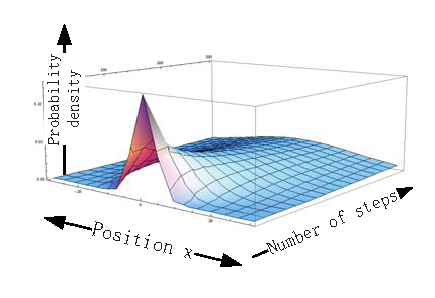
\includegraphics[width=8cm]{Fig_3} %	** if .eps don't need extension
\caption{The probability distribution of the classical random with the position and number of step. From the picture we know that as the number of steps increase, the walker will diffuse to all the lattice points, this character is used by many computer algorithm, although it is still has the max probability to be at the center.}\label{myfigure3}
\end{figure}

\begin{figure}[htb]	% h-here, t-top, b-bottom
\centering
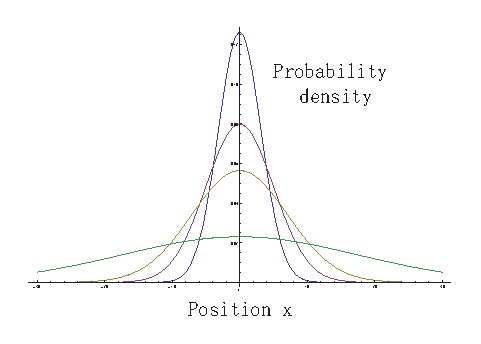
\includegraphics[width=8cm]{Fig_4} %	** if .eps don't need extension
\caption{For some special steps of the probability distribution of the classical random walk. (green: T=300; yellow: T=50; red: T=25; blue: T=10 )}\label{myfigure4}
\end{figure}

\subsection{Coined quantum walk}
Since classical random walk has been applied to many fields such as Brownian motion, randomized algorithm etc., we have enough reason to quantize the classical random walk to get more applications with the same advantages as quantum computer to classical computer because the superposition principle of quantum mechanics. This was done by Y. Aharonov, L. Davidovich, and N. Zagury in 1993 (\cite{Aharonov93}).

For an intuitional view, the quantum walk can be viewed as the quantization of the classical random walk. In the classical random walk, the walker can go to only one lattice at a time, in contrast, in quantum walk the walker can turn to both sides until be measured. It is showed as Fig. \ref{myfigure5}.
\begin{figure}[htb]	% h-here, t-top, b-bottom
\centering
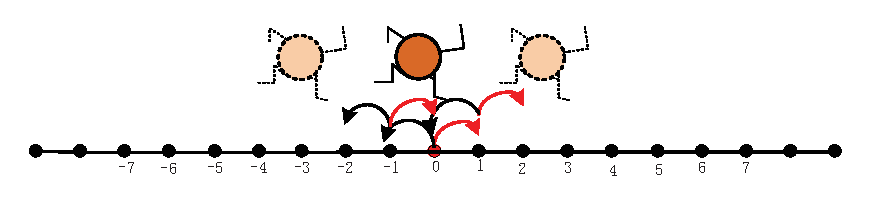
\includegraphics[width=8cm]{Fig_5} %	** if .eps don't need extension
\caption{The illustration of quantum walk in a intuitionistic way, we can consider the walker to go to the left and right simultaneously, this is one of the most amazed results of quantum mechanics, which was first illustrated by Feynman with the tool of path integral. This picture comes from (\cite{Kendon07})}\label{myfigure5}
\end{figure}

Formally, we should define the quantum walk in Hilbert space. Also for simplify we focus on the one dimensional lattice.

In the coined quantum walk, we should define two Hilbert space-the coin space and the position space:
\begin{equation}\label{myequation3}
H = H_c  \otimes H_p
\end{equation}

Where Hc is the coin Hilbert space and Hp is the position space, they have form as follow:
\begin{equation}\label{myequation4}
H_p  = \{ \left| x \right\rangle ;x \in \mathbb{Z}\} \begin{array}{*{20}c}
   {}  \\

 \end{array} ,H_c  = \{ \left| { + 1} \right\rangle ,\left| { - 1} \right\rangle \}
\end{equation}

Where \emph{x} is the position and can only be valued as integers, in the coin space +1 means go to right and -1 means go to left. In quantum walk, the walking process can be realized by the shift operator is defined as :
\begin{equation}\label{myequation5}
S = \left| { + 1} \right\rangle \left\langle { + 1} \right| \otimes \sum\limits_x {\left| {x + 1} \right\rangle } \left\langle x \right| + \left| { - 1} \right\rangle \left\langle { - 1} \right| \otimes \sum\limits_x {\left| {x - 1} \right\rangle } \left\langle x \right|
\end{equation}

And the coin operator is :
\begin{equation}\label{myequation6}
C = \left( {\begin{array}{*{20}c}
   a & b  \\
   c & d  \\

 \end{array} } \right)
\end{equation}

The \emph{S} operator and the \emph{C} operator are all unitary and hermitian, so for each step the evolution of the coin and space is also unitary as follow :
\begin{equation}\label{myequation7}
U = S(C \otimes I)
\end{equation}

As the same with the classical random walk, the quantum walk should be at a position before walking, but the initial condition of quantum walk can be very different from the classical random walk. The state of the coin in quantum walk can be superposition of the up and down, this makes it different from the classical random walk. The initial condition in quantum walk can be the form as follow :
\begin{equation}\label{myequation8}
\left| {\Psi _{in} } \right\rangle  = (\alpha \left| { + 1} \right\rangle  + \beta \left| { - 1} \right\rangle ) \otimes \left| x \right\rangle
\end{equation}

After \emph{T} step, the final state before measurement is :
\begin{equation}\label{myequation9}
U^T \left| {\Psi _{in} } \right\rangle
\end{equation}

Then we can perform the measurement of the position of the walker and get the position distribution according to the quantum mechanical rule.

As a example, we can set two quantum register: the coin register and the position register. The coin register has two possible state |+1> or |-1>, and the position register can be the state |x>, where \emph{x} is a integer.

The walking process is flip the coin first and then shift, we can set the coin operator as:
\begin{equation}\label{myequation10}
C = \frac{1}
{{\sqrt 2 }}\left( {\begin{array}{*{20}c}
   1 & 1  \\
   1 & { - 1}  \\

 \end{array} } \right)
\end{equation}

Flip the coin is :

$|+1>\rightarrow(|+1>+|-1>)/\sqrt{2}$

$|-1>\rightarrow(|+1>-|-1>)/\sqrt{2}$

Shift is :

$|+1>|x>\rightarrow|+1>|x+1>$

$|-1>|x>\rightarrow|-1>|x-1>$

We can also understand why the quantum walk is different from the classical random walk with the help of path integral method as Fig. \ref{myfigure6} (\cite{Perez Delgado07}).

If we plot the time axis, then the one dimensional lattice and the time form a two dimensional space, in figure 6, the dotted line is all the possible path and the real line is one of them, in classical random walk, the walker can only select one of the paths to walk, but in quantum walk the walker can walk in all possible paths simultaneously, the probability amplitude of every path can then interfere to each other.
\begin{figure}[htb]	% h-here, t-top, b-bottom
\centering
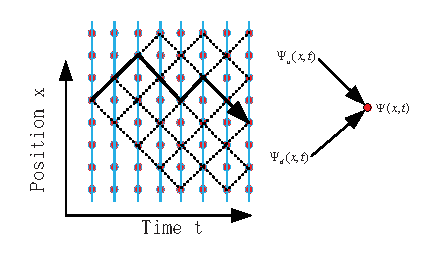
\includegraphics[width=8cm]{Fig_6} %	** if .eps don't need extension
\caption{ illustration of the quantum walk with the tool of path integral (\cite{Perez Delgado07}). We can plot both the time and the position axis, the red point stands for the lattice and the dotted line is all the possible path. In classical random walk, the walker can only choose one of the paths (the real line) with a probability, but in quantum walk one can walk in all possible paths simultaneously, the probability amplitude of every path can then interfere to each other if allowed.}\label{myfigure6}
\end{figure}

If the initial state of the coin is |-1>, then we can get the possibility distribution as Fig. \ref{myfigure7}.
\begin{figure}[htb]	% h-here, t-top, b-bottom
\centering
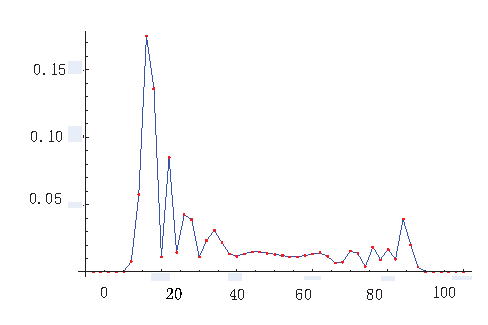
\includegraphics[width=8cm]{Fig_7} %	** if .eps don't need extension
\caption{Probability distribution of quantum walk with the initial state of the coin of |-1>, in this picture the walker start at the position x=50. The steps of this picture is 50}\label{myfigure7}
\end{figure}

Otherwise if we set the initial state of the coin to $\frac{1}
{{\sqrt 2 }}(\left| { + 1} \right\rangle  + i\left| { - 1} \right\rangle)$, then the possibility distribution is as Fig. \ref{myfigure8}. This is very different from classical random walk whose possibility distribution is independent of the initial conditions, which show the unitary of quantum mechanics.
\begin{figure}[htb]	% h-here, t-top, b-bottom
\centering
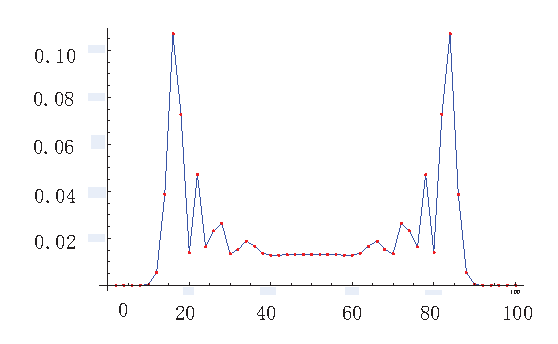
\includegraphics[width=8cm]{Fig_8} %	** if .eps don't need extension
\caption{Probability distribution of quantum walk with another initial state of the coin of $\frac{1}
{{\sqrt 2 }}(\left| { + 1} \right\rangle  + i\left| { - 1} \right\rangle$, in this picture the walker start also at the position x=50. compared with the figure 7 we can easily find that the probability distribution of quantum walk depends on the initial state of the coin, this is also different from the classical random walk, whose probability distribution is independent of the initial state of the coin.}\label{myfigure8}
\end{figure}
Another difference of quantum walk from classical random walk is the diffusion rate of the walker from the center, as we know from section 2.1, the deviation of the walker is proportional to the root of the step number N, but in quantum walk, the deviation of the walker is proportional to N, which get a quadric speed up(for a detail see the Fig. \ref{myfigure9}.
\begin{figure}[htb]	% h-here, t-top, b-bottom
\centering
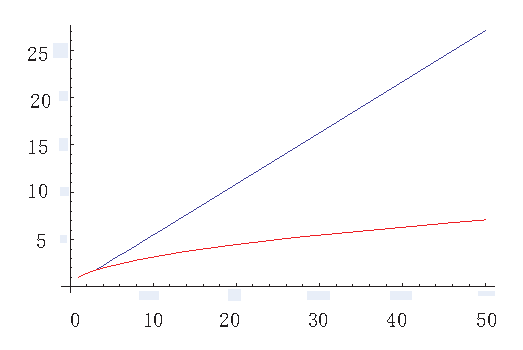
\includegraphics[width=8cm]{Fig_9} %	** if .eps don't need extension
\caption{The diffusion rate of the walker from the center, it can be characterized by the deviation of the walker's position from the center (i.e. the start place of the walker). The horizontal axis represents the number of the step \emph{T} and the vertical axis represents the deviation of the position. In this picture the gray line is the case of quantum walk and the red line is the case of the classical random walk. It can be concluded that the diffusion rate of the quantum walk is quadratic speed up upon the classical random walk.}\label{myfigure9}
\end{figure}
\subsection{Continues time quantum walk}
Continues time quantum walk is introduced by Edward Farhi and Sam Gutmann in 1998 (\cite{Farhi98}), in contrast with the coined quantum walk, the continues quantum walk does not need a coin, and is often defined with the tool of graphs.

It is convenient to illustrate the continues time quantum walk begin with the classical random walk on a graph, the process can be described by a matrix \emph{M}, which transform the probability distribution on the vertex of graph, the process is as follows:
\begin{equation}\label{myequation11}
p_i^{t + 1}  = \sum\limits_j {M_{ij} p_j^t }
\end{equation}

where $M_{ij}$ is the matrix element of M, and  is the probability at the i th vertex at the time t.

The next step is to make the transform process continuous, this require to jump to only the neighbor vertex, then we should use the infinitesimal generator matrix H to describe the walk process, i.e.
\begin{equation}\label{myequation12}
\frac{{dp_i (t)}}
{{dt}} =  - \sum\limits_j {H_{ij} p_j (t)}
\end{equation}

Solve the equation we get:
\begin{equation}\label{myequation13}
p(t) = \exp ( - Ht)p(0)
\end{equation}

Where p is the vector of probability distribution.

Then we can find the equation (\ref{myequation12}) has the similiar form with the Schr\"{o}dinger equation, so the classical random walk is quantized in a continues form.

\section{Search algorithm via quantum walk}
In section 2.2  we have know that in one dimensional lattice the walker depart from the center quadratically faster than classical random walk, however it is not a search process. But search is the reverse process: start in a uniform superposition of all the database and return to the marked item, so it is not difficult to understand why the quantum walk based search algorithm is quadratic speed up upon the classical search algorithm. Generally coined quantum walk can  make quantum walk faster than the continues time quantum walk( \cite{Ambainis05}).

Quantum walk can also be simulated by quantum circuit( \cite{Douglas09}), thus we can realized the quantum based search algorithm by the quantum computer in principle, this make quantum walk not a conceived tool for algorithm, then can be useful for the computation theory to explorer more efficient algorithms for intractable problems, for a review of the algorithm application of quantum walk we can see the article of Andris Ambainis and Vivien M Kendon ( \cite{Ambainis03,Kendon06})

\subsection{Searching on graphs}
In this subsection we will focus on the search on graphs. Searching on graphs is finding a marked vertex of the graph. Sometimes one is also interested in finding a marked edge or even a marked subgraph, which is generalized from the search of vertex.

Searching on the graph can be done by coined quantum walk (\cite{Shenvi03}) or continues time quantum walk (\cite{Childs04}), we will focus on the coined quantum walk based search algorithm most of the time. Hitherto the quantum walk is all defined on highly symmetric graphs such as hypercube.

In section 2.2 we have introduced the coined quantum walk on one dimensional lattice just for illustration, in order to interpret the search algorithm via quantum walk it is necessary to get the define of quantum walk on graph. This will be showed with the example of hypercube of dimension n. The first quantum walk based search algorithm is discovered by Neil Shenvi, Julia Kempe, and K. Birgitta Whaley ( \cite{Shenvi03}), which is called SKW algorithm. As a general example we will illustrate the SKW algorithm without loss of generality.

On higher dimensional graph, the only different from the quantum walk on a line is the dimension of the Hilbert space of coin and position. In graph the position is replaced by the vertex and the dimension of the coin Hilbert space is the degree of the graph.
For a n dimensional hypercube, the degree of every vertex is n and the number of the total nodes is $N = 2^n $, thus the Hilbert space of the vertex and coin is:
\begin{equation}\label{myequation14}
H = H_v  \otimes H_c
\end{equation}
Where Hv is the vertex space and Hc is the coin space which have the form:
\begin{equation}\label{myequation15}
H_v  = \{ \left| x \right\rangle :x \in \mathbb{Z}_N \}
\end{equation}
\begin{equation}\label{myequation16}
H_c  = \{ \left| c \right\rangle :c \in \mathbb{Z}_d \}
\end{equation}
Where N is the number of the total nodes and d is the degree of every vertex.

Then we can define the coin operator and the shift operator on the Hilbert space of the coin and vertex, they can take the form as follows (\cite{Shenvi03}):
\begin{equation}\label{myequation17}
S = \sum\limits_{d = 0}^{n - 1} {\sum\limits_{\vec x} {\left| {d,\vec x \oplus \vec e_d } \right\rangle } } \left\langle {d,\vec x} \right|
\end{equation}
\begin{equation}\label{myequation18}
C = C_0  \otimes I
\end{equation}

Where $\vec e_d$is the dth basis vector on the hypercube. $C_0$ is a $n \times n$ unitary operator acting on the coin space and I is an identity operator.
To implement the search algorithm it is natural to apply a marked coin operator, in the SKW algorithm for instance the marked coin operator is as follows:
\begin{equation}\label{myequation19}
C^\prime = C_0  \otimes I + (C_1  - C_0 ) \otimes \left| {\vec 0} \right\rangle \left\langle {\vec 0} \right|
\end{equation}
The marked coin can be any n��n unitary operator, for detail information we can see the literature (\cite{Shenvi03}).

The more generalized searching target on the graph can be a edge or even a subgraph (\cite{Hilley09}), Element distinctness is another algorithm that can be view as a quantum walk based search ( \cite{Ambainis07})

\subsection{Searching the exits}
Another algorithm of search using quantum walk is found by Andrew M. Childs et al in 2003, which is also the first quantum walk based algorithm. This algorithm use the exponential speed up of hitting time of quantum walk upon classical random walk ( \cite{Childs03}).
Contrast of the unsorted database, the algorithm found by Andrew M. Childs et al. is based on a particular sort of network (Fig. \ref{myfigure10}). Suppose that we are at the entrance of the network, our task is to find another exit as fast as possible. For classical case the best strategy may be to choose a direction randomly, i.e. the classical random walk. It still takes the time exponent increase with the wide of the network. You may be lost in the middle of the network. In quantum walk, however, one can choose all the possible paths simultaneously and reach the exit with the time increase polynomial with the wide of the network, which make a exponent speed up.
\begin{figure}[htb]	% h-here, t-top, b-bottom
\centering
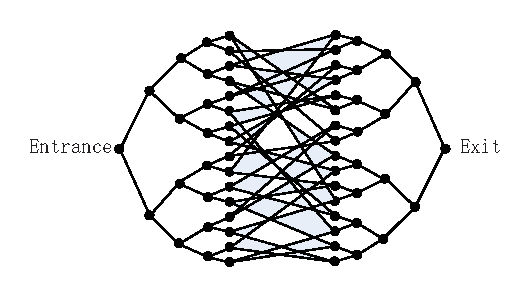
\includegraphics[width=8cm]{Fig_10} %	** if .eps don't need extension
\caption{ The network of the first algorithm found by Andrew M. Childs et al. that is based on quantum walk ( \cite{Childs03}). }\label{myfigure10}
\end{figure}

\section{Physical implementation of quantum walk based search}

\subsection{Introduction to the SKW algorithm}
The quantum random walk search algorithm proposed by Shenvi, Kempe and Whaley (SKW algorithm, \cite{Shenvi03}) is one of the novel algorithms which exhibit the superiority of quantum computation. It belongs to the discrete-time quantum random walk model. Similar to Grover's quantum search algorithm, the SKW algorithm performs an oracle search on a database of \emph{N} items with $O(\sqrt{\emph{N}})$ calls, where \emph{N} is the size of the search space. Whereas, when the diffusion step of Grover's algorithm cannot be implemented efficiently, this algorithm may be still available, which is a significant advantage comparing to the Grover's algorithm. Afterwards various optimizations of the SKW algorithm have been brought up to reduce the complexity (\cite{Ambainis05,Tulsi08,Reitzner09,Chandrashekar08}).

The original problem can be described as follows: given a function $\emph{f}\left(\emph{x}\right)$, $\emph{f}\left(\emph{x}\right)=1$ if $\emph{x}=\emph{a}$, otherwise $\emph{f}\left(\emph{x}\right)=0$. The goal is to find \emph{a}, where $0\leqslant \emph{a}\leqslant 2^n-1$. It is equivalent to search for a single marked node among the $\emph{N}=2^n$ nodes on the n-cube.

The discrete-time quantum random walk model requires a flipping coin and defines a two-step procedure consisting of a coin-flip step and coin-controlled walk step. The two steps can be expressed as $U=SC$, where $C$ denotes a unitary operation corresponding to flipping the quantum coin (coin-flip step) and $S$ is a permutation matrix which performs a controlled shift based on the state of the coin space (coin-controlled walk step). Specially, in the SKW algorithm, an oracle is needed to realize the searching procedure. The oracle acts by applying a marking coin $C_1$ to the marked node and the original
coin $C_0$ to the unmarked nodes, which is defined as a new coin operator $C'$. After applying $U'=SC'$ for $t_{f}=\frac{\pi}{2}\sqrt{2^n}$ times, we gain the marked node
with probability $\frac{1}{2}-O(1/n)$ by measurement.

A simple case for $n=2$ is considered. We need three qubits to demonstrate the algorithm, with one coin qubit (labeled by qubit 0) and two database qubits (labeled by qubit 1 and 2). The target node is one of the four computational bases ${\left\vert 00 \right\rangle_{12},\left\vert 01
\right\rangle_{12},\left\vert 10 \right\rangle_{12},\left\vert 11
\right\rangle_{12}}$, named by 1-out-of-4 algorithm. The network is shown in Fig.\ref{net}. Now we describe the searching process in details. Suppose the initial state is a pure state $\left\vert 000 \right\rangle$.

\begin{figure}[h] \centering
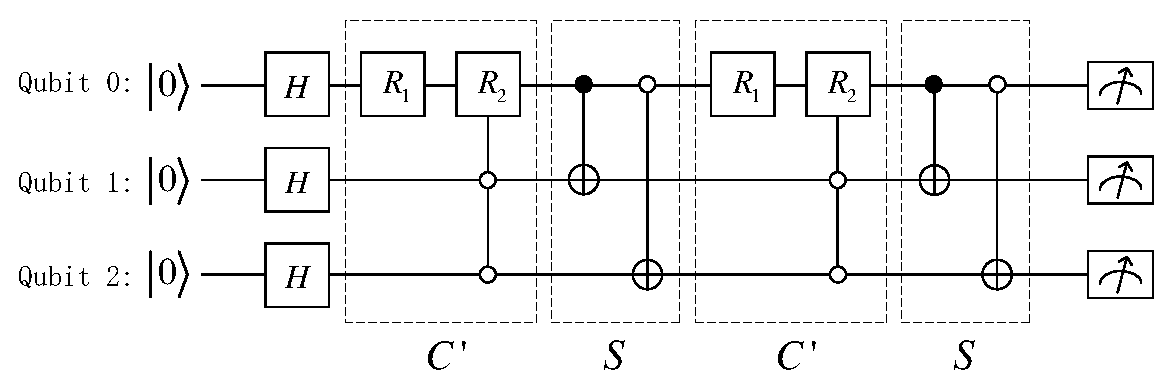
\includegraphics[width=\columnwidth]{net.eps}
\caption{\footnotesize{Quantum network for the algorithm of
1-out-of-4 searching, with the target state being $\left\vert 00
\right\rangle_{12}$. Qubit 0 is the coin qubit, while qubit 1 and 2 are database qubits.
The Hadamard gates are applied to produce an equal superposition over all the computational bases.
The solid circle represents 1-control gate whereas
the open circle represents the opposite. The purpose of oracle $C'$ is to implement
$C_1=R_x^0(\pi/2)$ (rotating qubit 0 around the \emph{x} axis by
angle $\pi/2$) when the database is $\left\vert 00
\right\rangle_{12}$ and $C_0=R_x^0(3\pi/2)$ otherwise. It is
equivalent to be replaced by $R_1=R_x^0(3\pi/2)$ and
$R_2=R_x^0(-\pi)$. The two controlled-not gates are inverting qubit
1 if qubit 0 is $\left\vert 1 \right\rangle_{0}$ and inverting qubit
2 if qubit 0 is $\left\vert 0 \right\rangle_{0}$, respectively. The
measurement requires all the populations'
reconstruction. Similar circuits can be obtained in a straightforward manner
for other target states. For instance, if the goal is $\left\vert 10
\right\rangle_{12}$, we need only change the controlled condition of
the three-body-interaction gate to state $\left\vert 10
\right\rangle_{12}$.}}\label{net}
\end{figure}

(I) Applying a Hadamard operation to every qubit to prepare the state
\begin{equation} \label{initial}
\left\vert \psi_{i} \right\rangle=\frac{\left\vert 0 \right\rangle_0+\left\vert 1 \right\rangle_0}{\sqrt{2}}\otimes\frac{\left\vert 0 \right\rangle_1+\left\vert 1 \right\rangle_1}{\sqrt{2}}\otimes\frac{\left\vert 0 \right\rangle_2+\left\vert 1 \right\rangle_2}{\sqrt{2}},
\end{equation}
which is exactly an equal superposition over all the computational bases.

(II) Perform the oracle $C'$ on the coin qubit
depending on the state of database qubits, namely,
$C_1=R_x^0(\pi/2)=e^{-i\pi\sigma_x/4}$ if the database qubits are
on the target state $\left\vert \tau\sigma \right\rangle_{12}$, and
$C_0=R_x^0(3\pi/2)=e^{-i3\pi\sigma_x/4}$ otherwise. Therefore, the
whole coin operation is
\begin{equation} \label{C'}
C'=C_0\otimes (E_{12}-\left\vert \tau\sigma
\right\rangle_{12\ 12}\left\langle \tau\sigma \right\vert)+C_1\otimes\left\vert \tau\sigma
\right\rangle_{12\ 12}\left\langle \tau\sigma \right\vert
\end{equation}
where $E_{12}$ is the identity operator.
Then the database qubits undergo the shift operation $S$
conditioned on the state of coin qubit:
\begin{eqnarray}\label{S}
&&\left\vert 0 \right\rangle_{0}\left\vert 00 \right\rangle_{12}\Longleftrightarrow\left\vert 0 \right\rangle_{0}\left\vert 01 \right\rangle_{12} \nonumber\\
&&\left\vert 0 \right\rangle_{0}\left\vert 10 \right\rangle_{12}\Longleftrightarrow\left\vert 0 \right\rangle_{0}\left\vert 11 \right\rangle_{12} \nonumber\\
&&\left\vert 1 \right\rangle_{0}\left\vert 00 \right\rangle_{12}\Longleftrightarrow\left\vert 1 \right\rangle_{0}\left\vert 01 \right\rangle_{12} \nonumber\\
&&\left\vert 1 \right\rangle_{0}\left\vert 01
\right\rangle_{12}\Longleftrightarrow\left\vert 1
\right\rangle_{0}\left\vert 11 \right\rangle_{12}
\end{eqnarray}

(III) Repeat step (II) twice to implement the quantum walk, which will reach the final state
\begin{equation}
\left\vert \psi_{f} \right\rangle=\left( SC' \right)^2 \left\vert \psi_{i} \right\rangle
\end{equation}

(IV) Measure all the populations of the database qubits.
For example, in the case of finding ${\left\vert 00 \right\rangle_{12}}$, we can obtain that the
probabilities of ${\left\vert 00 \right\rangle_{12},\left\vert 01
\right\rangle_{12},\left\vert 10 \right\rangle_{12},\left\vert 11
\right\rangle_{12}}$ are 0.5, 0.25, 0.25, 0, respectively.

For other target states, with the controlled condition changed to the target node similar networks can be given easily. The results have an analogy with the aforementioned one.

\subsection{NMR experimental implementation}

Now we turn to our NMR quantum computer to implement the SKW algorithm. The three qubits are represented by the three ${}^1$H spins in a
sample of 1-Bromo-2,3-Dichlorobenzene oriented in liquid-crystal
solvent (ZLI-1132). The molecular structure is shown in Fig.\ref{energy_level}(a). The system Hamiltonian can be described as
\begin{eqnarray}\label{Hamiltonian}
\mathcal{H}=&&\sum\limits_{j=1}^3 {2\pi \nu _j } I_z^j  + \sum\limits_{j,k,j < k\leqslant 3} {2\pi} J_{jk} (I_x^j I_x^k  + I_y^j I_y^k+I_z^j I_z^k) \nonumber\\
&&+ \sum\limits_{j,k,j < k\leqslant 3} {2\pi} D_{jk} \left( {2I_z^j I_z^k  - I_x^j I_x^k  - I_y^j I_y^k } \right)
\end{eqnarray}
where $\nu_j$ is the resonance frequency of the \emph{j}th spin,
$\emph{D}_{jk}$ and $\emph{J}_{jk}$ are the dipolar coupling
strengths and scalar coupling strengths between spins \emph{j} and
\emph{k}, respectively. All the sums are restricted to the spins within one molecule. All experiments were carried out on a Bruker Avance
500 MHz spectrometer at room temperature. The spectrum of the thermal equilibrium state
$\rho_{th}=\sum\limits_{i=1}^3 \sigma_z^i$ followed by a $\pi/2$
hard pulse is shown in Fig.\ref{energy_level}(b). With some
initially guessed parameters assuming the molecular geometry, we iteratively fit the
calculated and observed spectra through the parameters'
perturbation (\cite{Suryaprakash00}). The values of parameters are listed in Table.\ref{para}(a).

\begin{figure}[h] \centering
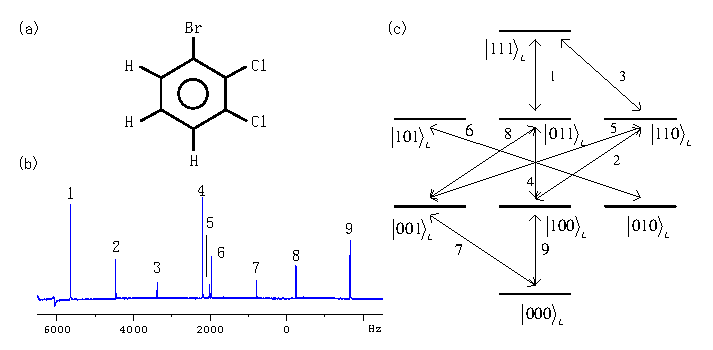
\includegraphics[width=\columnwidth]{energy_level.eps}
\caption{\footnotesize{(a) Molecular structure of
1-Bromo-2,3-Dichlorobenzene in which the three protons form a 3-qubit
system. (b) Spectrum of the thermal equilibrium state
followed by a $\pi/2$ hard
pulse. All the observable transitions are labeled according to the descending
orders of the frequencies. (c) Diagram of corresponding
transitions in the eigenbasis.}}\label{energy_level}
\end{figure}

\begin{table}[htb] \centering
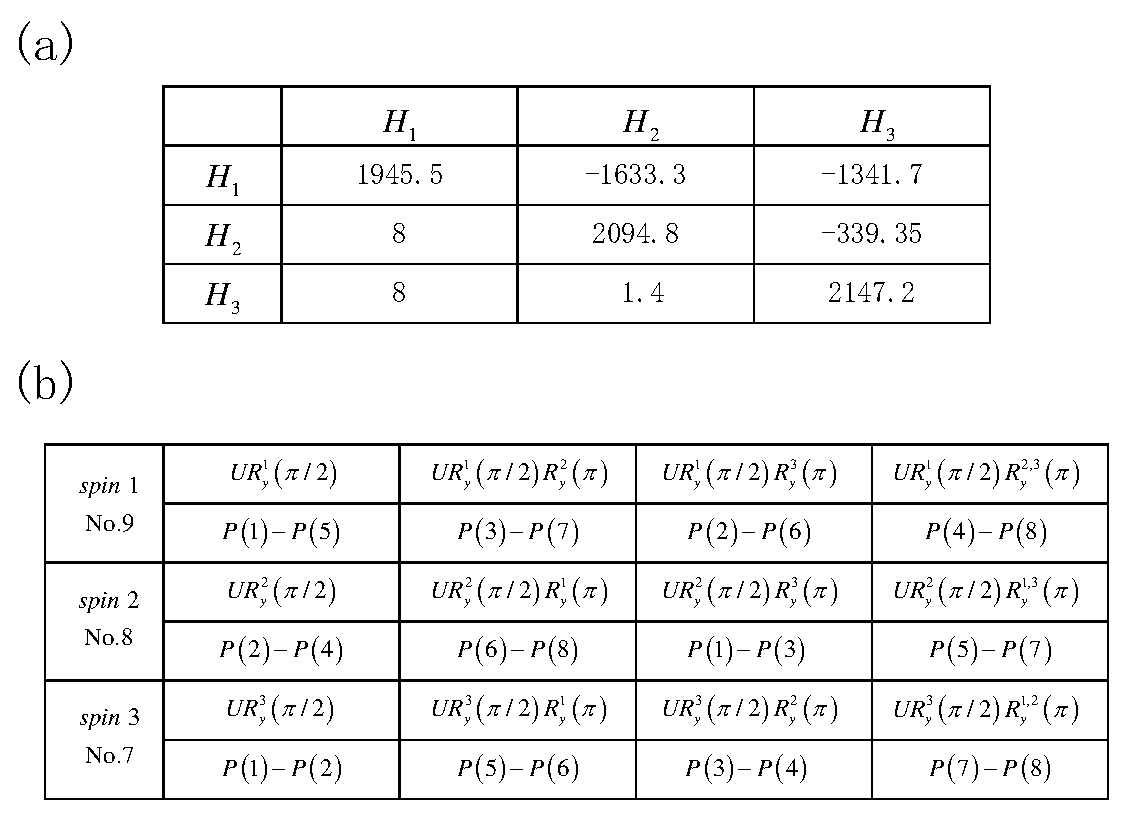
\includegraphics[width=0.9\columnwidth]{para.eps}
\caption{\footnotesize{(a) The parameters for fitting the spectrum of
1-Bromo-2,3-Dichlorobenzene (Hertz). The diagonal elements are chemical
shifts of the three protons, the upper-right off-diagonal elements
are dipolar coupling strengths, and the lower-left ones are scalar
coupling strengths. (b) The read-out pulses and corresponding values
of $P(i)-P(j)$. The results are shown on the transitions of No.9, 8
and 7.}}\label{para}
\end{table}

Since the system Hamiltonian has nondiagonal elements, the eigenstates are not Zeeman product states any more but linear combinations of them. To simplify the measurement of populations (marked from $P(1)$ to $P(8)$), we found a feasible unitary matrix \emph{U} to realize the transformation between the computational basis and eigenbasis, which satisfies
\begin{equation} \label{diag}
H_L = UH_SU^{\dag},
\end{equation}
where $H_S$ is the system Hamiltonian and $H_L$ is a diagonal
Hamiltonian (i.e., the Hamiltonian in the eigenbasis). With adding the pulse of implementing transformation matrix \emph{U} after the original readout pulses in liquid NMR and combining with the normalization $\sum_{i=1}^8P(i)=1$, we can obtain all eight population values straightforwardly. Table. \ref{para} (b) shows all the
available values of $P(i)-P(j)$ through different read-out pulses (for more explanations and details see \cite{Lu10}.

The experiment was divided into three steps: the psesudo-pure state
preparation, quantum random walk searching process, and population
measurement. Starting from the thermal equilibrium state, firstly we
need to create the PPS $\rho_{000}=\frac{1-\epsilon
}{8}\mathbf{1}+\epsilon \left\vert 000 \right\rangle \left\langle
000\right\vert$, where $\epsilon$ represents the polarization of the
system and $\mathbf{1}$ is the identity matrix. We used shape pulses based on GRadient Ascent Pulse Engineering (GRAPE)
algorithm (\cite{Khaneja05,Baugh07,Ryan08}) and gradient pulses to realize the PPS
preparation, with the numerical simulated fidelity 0.977.

The quantum random walk searching process contains two parts
actually: The preparation of initial state $|+\rangle^{\otimes3}$
($|+\rangle=(|0\rangle+|1\rangle)/\sqrt{2}$) and two iterations of
unitary evolution. We packed them together and calculated one GRAPE
pulse of 20ms and 250 segments whose fidelity is higher than 0.990. The reading-out operators listed in Table.\ref{para}(b) are also performed when generating the GRAPE pulses of 20ms with the fidelity 0.990. The probabilities of gaining $\left\vert 00
\right\rangle$, $\left\vert 01 \right\rangle$, $\left\vert
10 \right\rangle$, $\left\vert 11 \right\rangle$ are
0.513, 0.232, 0.197, and 0.058, respectively, which demonstrates that we have completed
searching $\left\vert 00 \right\rangle$ based on the SKW
algorithm.

Besides $\left\vert 00 \right\rangle$, we altered the target
states to $\left\vert 01 \right\rangle$, $\left\vert 10
\right\rangle$ and $\left\vert 11 \right\rangle$. The
experimental results are plotted in Fig.
\ref{result}. It can be seen the experimental and theoretical
results are mostly consistent with little error. The slight
difference between theory and experiment may be attributed to
decoherence, the RF field inhomogeneity and imperfect implementation of GRAPE pulses.

\begin{figure}[h] \centering
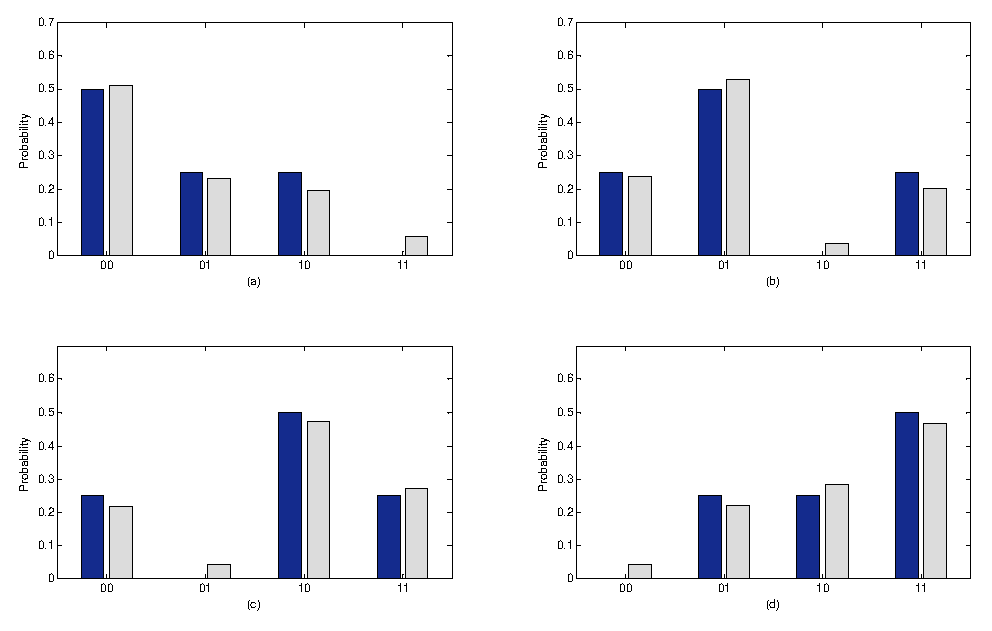
\includegraphics[width=\columnwidth]{result.eps}
\caption{\footnotesize{Experimental results of the SKW algorithm.
(a), (b), (c), (d) correspond to the cases of
finding $\left\vert 00 \right\rangle_{12}$, $\left\vert 01
\right\rangle_{12}$, $\left\vert 10 \right\rangle_{12}$ and
$\left\vert 11 \right\rangle_{12}$. The blue (dark) bars represent the
theoretical prediction and the gray (light) bars represent the experimental
analog, respectively. }}\label{result}
\end{figure}

In summary, we experimentally implemented a search algorithm based on the quantum random walk (the SKW algorithm) in the case of 1-out-of-4. This algorithm performs an oracle search on a database of N items with $O(\sqrt{N})$ calls, with a speedup similar to the Grover search algorithm. The experiment was carried out on an NMR quantum information processor with strongly dipolar coupled spins. We used GRAPE pulses to realize high-fidelity unitary operations and provided an effective way to measure the populations of the density matrix. The experimental results agree well with the theoretical expectations, which exhibits the superiority of the algorithm.

\section{Quantum walk based search in nature}
One of the astonishing phenomena of nature is the photosynthesis, which supply all the chemical energy of our earth and act as a important form of energy storage. However the high efficiency of the energy transfer in photosynthesis is still a enigma, the method of quantum walk has been introduced to try to explain the process of energy transfer (\cite{Mohseni08,Rebentrost09}) since the quantum walk can increase the search efficiency with exponentially speed up in the case of the uncharted network (\cite{Childs03}). Also in some literature the search process in photosynthesis from the pigment antenna to the reaction center is compared with the Grover type search, it is more natural to use the algorithm of section 3.2 to explain the high efficiency of the energy transfer process.
\subsection{Photosynthesis and quantum walk}
In photosynthesis the energy is absorbed by pigments and then transferred to the reaction center where the energy is converted to the chemical energy and start the electron transfer process. The most model of the energy transfer from the antennas to the reaction center is as the Fig. \ref{myfigure16} (\cite{Blankenship02}). In the past the popular view is the excitons from the antennas hop to the reaction center, which is analog to the classical random walk. However this is challenged by recent experiments and theory model, the quantum coherence is applying to the energy transfer process in order to explain the high efficiency in photosynthesis.
\begin{figure}[htb]	% h-here, t-top, b-bottom
\centering
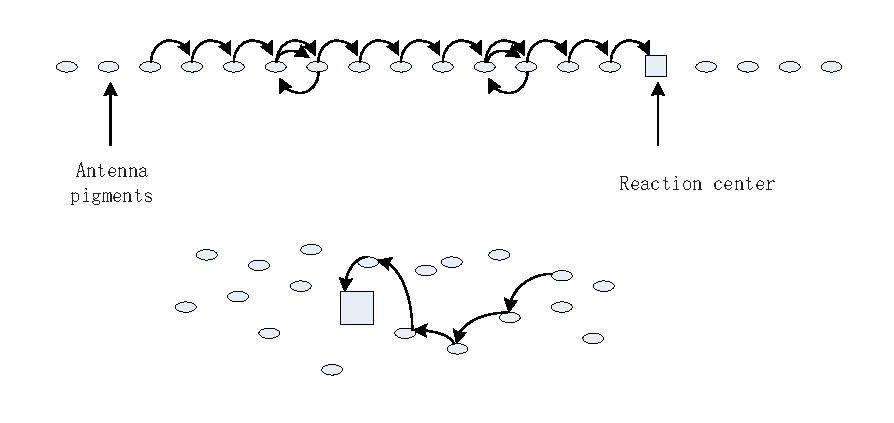
\includegraphics[width=8cm]{Fig_16} %	** if .eps don't need extension
\caption{Antenna organization models. The circle represents the antennas and the rectangle acts as the reaction center. The top schematic is the one dimensional array and the bottom schematic is the three dimensional array model. Of course the three dimensional model is more close to the actual case. The schematic come from the book written by Robert E. Blankenship. (\cite{Blankenship02})}\label{myfigure16}
\end{figure}

The first wavelike energy transfer though quantum coherence is found in FMO protein complex  of purple bacteria at the temperature of 77K (\cite{Engel07}) and soon the long lived quantum coherence in photosynthetic complexes is observed at physiological temperature (\cite{Panitchayangkoon10}).

The theory model of the energy transfer in photosynthesis is using the quantum walk (\cite{Mohseni08,Rebentrost09}), at most of the time the array of the pigment can be treated as a graph network of quantum walk (Fig. \ref{myfigure17} ), in the figure the red sites is just as the exits of the Fig. \ref{myfigure10} and the gray sites act as the entrance.

Another astonishing result is the assist of the environment to the quantum walk transport in photosynthetic energy transfer, if we know that environment is the main source of the decoherence of quantum systems and the decoherence is the main obstruct to build a quantum computer that surpass the classical computer. In contrast the interaction of the free Hamiltonian of the protein complex with the thermal fluctuations in the environment leads to a increase of the energy transfer efficiency from about 70\% to 99\% (\cite{Mohseni08}).
\begin{figure}[htb]	% h-here, t-top, b-bottom
\centering
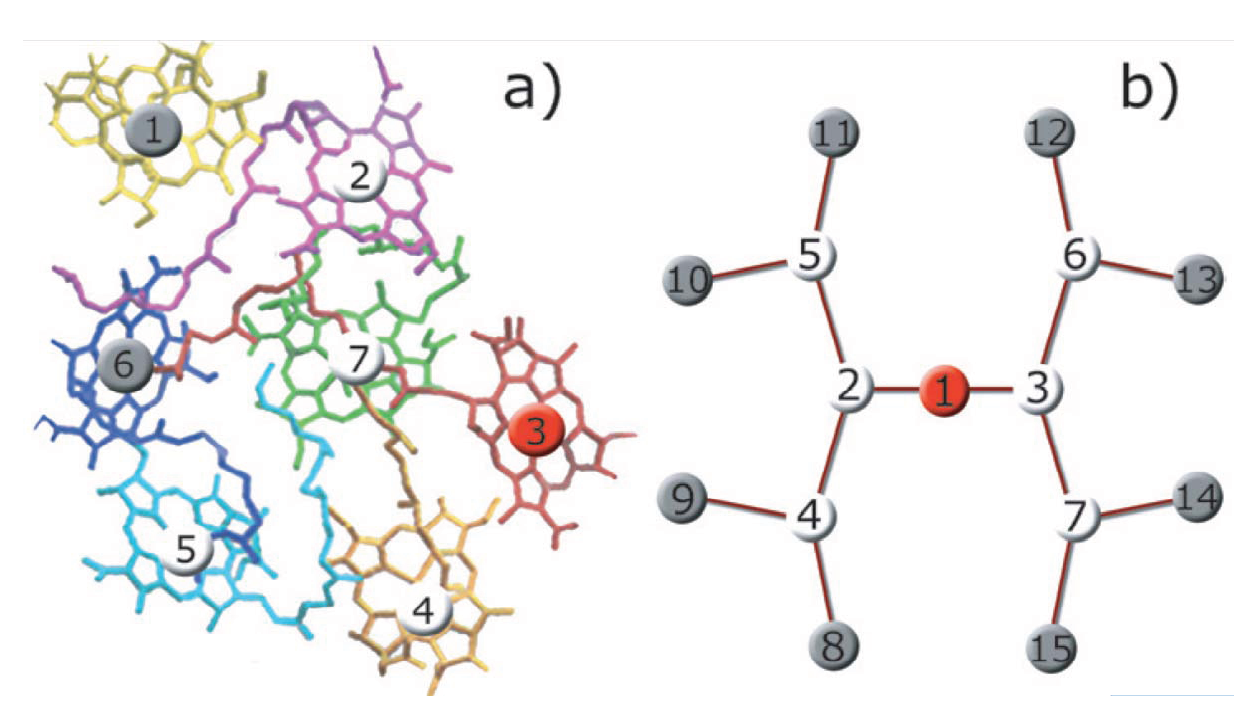
\includegraphics[width=8cm]{Fig_17} %	** if .eps don't need extension
\caption{a) chlorophyll molecules Fenna-Matthews-Olson (FMO) protein complex, this is investigated widely for its simple structure compared with the chlorophyll molecules in higher plant and algae.  b) artificial systems described by a tight-binding Hamiltonian. Here is a four generation  binary  tree. In  particular,  an  exponential  speed  up  in reaching certain target sites (red) in these structures has been proposed in the context of quantum walk algorithms. (The gray sites represent initial states for the quantum transport.) (\cite{Rebentrost09})}\label{myfigure17}
\end{figure}

\subsection{Biomimetic application in solar energy}
Energy is a crucial problem for human since the fossil fuels are being exhausted. A commonly accepted alternative energy assuming way is to use the solar energy directly, since it can be got continuously. However the efficiency of the solar energy used now is still very low, on the other way the efficiency of the energy transfer in the photosynthesis is very high: more than 90\% sometimes upon to 99\%. If the energy transfer efficiency in the solar cell achieve to the same as in photosynthesis then the conversion efficiency of solar cell will double up. This will give a exited perspective to the future of the energy utilization of human if we can understand the principle of the energy transfer in photosynthesis. Hitherto many group have committed to build a artificial photosynthesis system, not successful enough however until now. Although many of them claim to be solve the puzzler of the energy in the earth, from a scientific view we cannot conclude when can we see the hydrogen emerge from the water extensive under the shine of the sun.

It is not necessary to list the benefit of the solar energy since there are so many eyes searching them, the only task for us is to make the principle of the photosynthesis clear so we can utilize it as we will do.

\section{Conclusions and future directions}
Quantum walk is another approach to design a quantum algorithm surpassing the classical algorithms, hitherto many scientists have made commitment to build a quantum computer. Apart from the search problem, there are many problems that can not be solved by classical computer efficiently, but they can be solved by quantum algorithms in a relative short time. Quantum walk is not just the artificial tool for the search algorithm, but is also likely to be the tool for nature. All of these are instilling confidence for us to solve the intractable problems we have met.

However, the main obstacle of the quantum walk based algorithms including the search algorithm is the physical implementation since the decoherence seems to be not solvable in the near future. Thus in the future our main purpose should be the overcoming of the decoherence or realizing the coherent manipulation of the quantum bits and quantum systems for relative long time in particular case. There are also many physical systems proposed to use to implement the quantum computer and the quantum walk, but which is the practical one to realize our dream of quantum computer is still unknown.

Quantum walk has been realized in various physical systems, first in NMR based computer (\cite{Du03})for continues time quantum walk and then coined quantum walk (\cite{Ryan05}). There are also many other physical systems such as waveguide lattices (\cite{Perets08}), trapped ions (\cite{Schmitz09,Zahringer10}), photon systems (\cite{Schreiber10,Broome10}) and optical lattices (\cite{Karski09}) in which quantum walk has been realized, but the number of step is still very small. May be the photons in waveguide lattice is a particular system since it has been used to realize the continues quantum walk for more than one hundred of steps, but this systems is not convenient to modulate the walker. Anyway we have taken a giant step to realize the quantum walk in physical systems after which we can run the various search algorithms basing on quantum walk.

\begin{thebibliography}{100}
\bibitem[Aharonov et al., 1993]{Aharonov93} Aharonov, Y. ; Davidovich, L. \& Zagury, N. (1993). Quantum random walks, \emph{ Phys. Rev. A }, \textbf{48}, 1687.
\bibitem[Ambainis, 2003]{Ambainis03} Ambainis, A. (2003). Quantum walks and their algorithmic applications, \emph{ International Journal of Quantum Information }, \textbf{1}, 507-518.
\bibitem[Ambainis, 2005]{Ambainis05} Ambainis, A.; Kempe, J. \& Rivosh, A. (2005). Coins Make Quantum Walks Faster,  \emph{ Proceedings of the 16th annual ACM-SIAM symposium on Discrete algorithms }, pp. 1099 - 1108  , 0-89871-585-7, Vancouver, British Columbia, 2005, Society for Industrial and Applied Mathematics.  Philadelphia.
\bibitem[Ambainis, 2007]{Ambainis07} Ambainis, A. (2007). Quantum walk algorithm for element distinctness, \emph{ SIAM Journal on Computing }, \textbf{37(1)}, 210-239.
\bibitem[Blankenship, 2002]{Blankenship02} Blankenship, R. E. (2002). \emph{Molecular Mechanisms of Photosynthesis}, Wiley-Blackwell, 978-0632043217, Oxford/ Malden.
\bibitem[Baugh et al., 2007]{Baugh07} Baugh, J. et al., (2007). 'Special issue on quntum information and quantum computing', \emph{Phys. in Can.} \textbf{63}, No.4.
\bibitem[Broome et al., 2010]{Broome10} Broome, M. A.; Fedrzzi, A.; Lanyon, B. P.; Kassal, I.; Apspuru-Guzik, A. \& White, A. G. (2010). Discrete Single-Photon Quantum Walks with Tunable Decoherence, \emph{Phys. Rev. Lett.} \textbf{104}, 153602.
\bibitem[Childs et al., 2003]{Childs03} Childs, A. M. ; Cleve, R. ; Deotto, E.; Farhi, E.; Gutmann, S. \& Speilman, D. A. (2003). Exponential algorithmic speedup by quantum walk,  \emph{ Proceedings of the thirty-fifth annual ACM symposium on Theory of computing }, pp. 59-68, 1-58113-674-9, San Diego, CA, USA, 2003, ACM, New York.
\bibitem[Childs \& Goldstone, 2004]{Childs04} Childs, A. M. \& Goldstone, J. (2004). Spatial search by quantum walk, \emph{ Phys. Rev. A }, \textbf{70}, 022314.
\bibitem[Chandrashekar, 2008]{Chandrashekar08} Chandrashekar, C.; Srikanth, R. \& Laflamme, R. (2008). Optimizing the discrete time quantum walk using a SU(2) coin, \emph{Phys.Rev. A} \textbf{77}, 032326.
\bibitem[Du et al., 2003]{Du03} Du, J. F.; Li, H.; Xu, X. D.; Shi, M. J.; Wu, J. H.; Zhou, X. Y.; \& Han, R. D. (2003). Experimental implementation of the quantum random-walk algorithm, \emph{Phys. Rev. A }, \textbf{67}, 042316.
\bibitem[Douglas \& Wang , 2009]{Douglas09} Douglas, B. L. \& Wang J. B. (2009). Efficient quantum circuit implementation of quantum walks, \emph{Phys. Rev. A }, \textbf{79}, 052335.
\bibitem[Engel et al., 2007]{Engel07} Engel, G. S. ; Calhoun, T. R.; Read, E. L.; Ahn, T. K.; Man\v{c}al, T.; Cheng, Y. C.; Blankenship, R. E.; \& Fleming, G. R. (2007). Evidence for wavelike energy transfer through quantum coherence in photosynthetic systems, \emph{Nature}, \textbf{446}, 782.
\bibitem[Farhi \& Gutmann, 1998]{Farhi98} Farhi, E. \& Gutmann, S. (1998). Quantum computation and decision trees, \emph{ Phys. Rev. A }, \textbf{ 58}, 915-928.
\bibitem[Grover, 1997]{Grover97} Grover, L. K. (1997). Quantum Mechanics Helps in Searching for a Needle in a Haystack, \emph{ Phys. Rev. Lett. }, \textbf{79}, 325-328.
\bibitem[Hilley et al., 2009]{Hilley09} Hilley, M.; Reitzner, D. \& Bu\v{z}ek, V. (2009). Searching via walking: How to find a marked subgraph of a graph using quantum walks, \emph{arXiv},  arXiv:0911.1102v1.
\bibitem[Kempe, 2003]{Kempe03} Kempe, J. (2003). Quantum random walks - an introductory overview, \emph{ Contemporary Physics }, \textbf{44 (4)}, 307-327.
\bibitem[Khaneja et al., 2005]{Khaneja05} Khaneja, N.; Reiss, T.; Kehlet, C.; Schulte-Herbr\"{u}ggen, T. \& S. Glaser. (2005). Optimal control of coupled spin dynamics: design of NMR pulse sequences by gradient ascent algorithms, \emph{J. Magn. Reson.} \textbf{172}, 296;
\bibitem[Kendon, 2006]{Kendon06} Kendon, V. M.; (2006). A random walk approach to quantum algorithms, \emph{ Phil. Trans. R. Soc. A }, \textbf{364}, 3407-3422.
\bibitem[Kendon et al., 2007]{Kendon07} Kendon, V. \&  Maloyer, O. (2007). Optimal computation with noisy quantum walks, \emph{ Quantum Information School of Physics $\&$ Astronomy University of Leeds Leeds LS2 9JT }.
\bibitem[Karski et al., 2009]{Karski09} Karski, M.; F\"{o}rster, L.; Choi, J. M.; Steffen, A.; Alt, W. \& Meschede, D. (2009). Quantum Walk in Position Space with Single Optically Trapped Atoms, \emph{Science} \textbf{325}, 174-177.
\bibitem[Lu et al., 2010]{Lu10} Lu, D.; Zhu, J.; Zou, P.; Peng, X.; Yu, Y.; Zhang, S.; Chen, Q. \& Du, J. (2010). Experimental implementation of a quantum random-walk search algorithm using strongly dipolar coupled spins, \emph{Phys. Rev. A} \textbf{81},022308.
\bibitem[Mohseni et al., 2008]{Mohseni08} Mohseni, M. ; Rebentrost, P. ; Lloyd, S. \& Aspuru-Guzik, A. (2008). Environment-assisted quantum walks in photosynthetic energy transfer, \emph{J. Chem. Phys.}, \textbf{129}, 174106.
\bibitem[P\'{e}rez Delgado, 2007]{Perez Delgado07} P\'{e}rez Delgado, C. A. (2007). Quantum Cellular Automata: Theory and Applications, \emph{ A thesis for the degree of Doctor of Philosophy in Computer Science },p61.
\bibitem[Perets et al., 2008]{Perets08} Perets, H. B.; Lahini, Y.; Pozzi, F.; Sorel, M.; Morandotti, R. \& Silberberg, Y. (2008). Realization of Quantum Walks with Negligible Decoherence in Waveguide Lattices, \emph{Phys. Rev. Lett.} \textbf{100}, 170506.
\bibitem[Poto\v{c}ek et al., 2009]{Potocek09} Poto\v{c}ek, V.; G\'{a}bris, A.; Kiss, T. \& Jex, I. (2009). Optimized quantum random-walk search algorithms on the hypercube, \emph{Phys. Rev. A} \textbf{79}, 012325.
\bibitem[Panitchayangkoon et al., 2010]{Panitchayangkoon10} Panitchayangkoon, G. ; Hayes, D.; Fransted, K. A.; Caram, J. R.; Harel, E.; Wen, J. Z.; Blankenship, R. W.;  \& Engel, S.  (2010). Long-lived quantum coherence in photosynthetic complexes at physiological temperature, \emph{Proc. Natl. Acad. Sci. USA }, \textbf{107}, 12766-12770.
\bibitem[Reichl, 1998]{Reichl98} Reichl, L. E. (1998). \emph{A Modem Course in Statistical Physics}, John Wiley \& Sons, Inc., 978-0471595205, New York.
\bibitem[Ryan et al., 2005]{Ryan05} Ryan, C.; Laforest, M.; \& Laflamme, R. (2005). Experimental implementation of a discrete-time quantum random walk on an NMR quantum-information processor, \emph{Phys. Rev. A} \textbf{72}, 012328.
\bibitem[Ryan et al., 2008]{Ryan08} Ryan, C.; Negrevergne, C.; Laforest, M.; Knill, E. \& Laflamme, R. (2008). Liquid-state nuclear magnetic resonance as a testbed for developing quantum control methods, \emph{Phys. Rev. A} \textbf{78}, 012328.
\bibitem[Reitzner et al., 2009]{Reitzner09} Reitzner, D.; Hillery, M.; Feldman, E. \& Bu\v{z}ek, V. (2009) Quantum searches on highly symmetric graphs,  \emph{Phys. Rev. A } \textbf{79}, 012323.
\bibitem[Rebentrost, 2009]{Rebentrost09} Rebentrost,P.; Mohseni, M.; Kassal, I.; Lloyd, S. \& Aspuru-Guzik, A. (2009). Environment-assisted quantum transport, \emph{New Journal of Physics }, \textbf{11}, 033003.
\bibitem[Suryaprakash, 2000]{Suryaprakash00} Suryaprakash, N. (2000). Liquid Crystals As Solvents in NMR: Spectroscopy Current Developments in Structure Determination, \emph{Current Organic Chemistry} \textbf{4}, 85-103.
\bibitem[Shenvi et al., 2003]{Shenvi03} Shenvi, N.; Kempe, J. \& Whaley, K. (2003). Quantum random-walk search algorithm, \emph{Phys. Rev. A} \textbf{67}, 052307.
\bibitem[Schmitz et al., 2009]{Schmitz09} Schmitz, H.; Matjeschk, R.; Schneider, C.; Gluechert, J.; Enderlein, M.; Huber, T. \& Schaetz, T. (2009). Quantum Walk of a Trapped Ion in Phase Space, \emph{Phys. Rev. Lett.} \textbf{103}, 090504.
\bibitem[Schreiber et al., 2010]{Schreiber10} Schreiber, A.;  Cassemiro, K. N.;  Poto\v{c}ek, V.;  G\'{a}bris, A.; Mosley, P. J.; Andersson, E.; Jex, I. \&  Silberhorn, C. (2010). Photons Walking the Line: A Quantum Walk with Adjustable Coin Operations, \emph{Phys. Rev. Lett.} \textbf{104}, 050502.
\bibitem[Tulsi, 2008]{Tulsi08} Tulsi, A. (2008). Faster quantum-walk algorithm for the two-dimensional spatial search, \emph{Phys. Rev. A} \textbf{78}, 012310.
\bibitem[Z\"{a}hringer et al., 2010]{Zahringer10} Z\"{a}hringer, F.; Kirchmair, G.; Gerritsma, R.; Solano, E.; Blatt, R. \& Roos, C. F. (2010). Realization of a Quantum Walk with One and Two Trapped Ions, \emph{Phys. Rev. Lett.} \textbf{104}, 100503.
\end{thebibliography}
%%% Without a bib file, write your references like this: **************
%\begin{thebibliography}{100}

%\bibitem[Arai \& Kragic, 1999]{arai99} Arai, T. \& Kragic, D. (1999). Name of paper, In: \emph{Name of Book in Italics}, Name(s) of Editor(s), (Ed.), page numbers (first-last), Publisher, ISBN, Place of publication

%\bibitem[Arkin, 2004]{arkin04} Arkin, D. (2004). \emph{My Life}, Arkin Publishing, Arkinson.

%\bibitem[Li et al., 1996]{li96} Li, B.; Xu, Y. \& Choi, J. (1996). Title of conference paper,  \emph{Proceedings of xxx xxx in italics}, pp. 14-17, ISBN, conference location, month and year, Publisher, City

%\bibitem[Lima et al., 2004]{lima04} Lima, P.; Bonarini, A. \& Mataric, M. (2004). \emph{Name of Book in Italics}, Publisher, ISBN, Place of Publication.

%\bibitem[Mataric \& Brooks, 1999]{mataric99} Mataric M. \& Brooks, R. (1999). To whom it may concern. \emph{Journal of Everything}, Vol. $\infty$, No. $\aleph_0$, Jan -1999, -10 -- -5, ISSN 00-XY-A

%\bibitem[Siegwart, 2001]{siegwart01} Siegwart, R. (2001). Name of paper. \emph{Name of Journal in Italics}, Vol., No., (month and year of the edition) page numbers (first-last), ISSN

%\bibitem[Siegwart et al., 2006]{siegwart06} Siegwart, R.; Gross, S.; Klein L. (2006). The Singularity has gone. \emph{Future beyond Science}, Vol. 0, No. 0, April 3000, 1--1 000 000, ISSN 00-0000-00-00Y

%\end{thebibliography}

%%% With a bib file, include it! *************************************
\bibliography{temp}

\end{document}
